\documentclass[10pt]{beamer}
\usetheme{jambro}

\title[]{Macroeconomia I - Apresentação}
\author[]{Paulo Victor da Fonseca}
\date{28 de fevereiro de 2023}

\hypersetup{
    colorlinks = true,
    urlcolor = teal,
    linkcolor = white    
}
\usepackage[portuguese]{babel}
\usepackage{subfig}
\usepackage{emoji}

\captionsetup[subfloat]{labelformat=empty}
\begin{document}
\begin{frame}[plain]
    \titlepage{
        \begin{center}
            \begin{minipage}{0.8\textwidth}
                \centering
            \end{minipage}
        \end{center}}
\end{frame}

\section{Docente}
\begin{frame}{Docente}
    \begin{tabular}{cl}
        \begin{tabular}{c}
            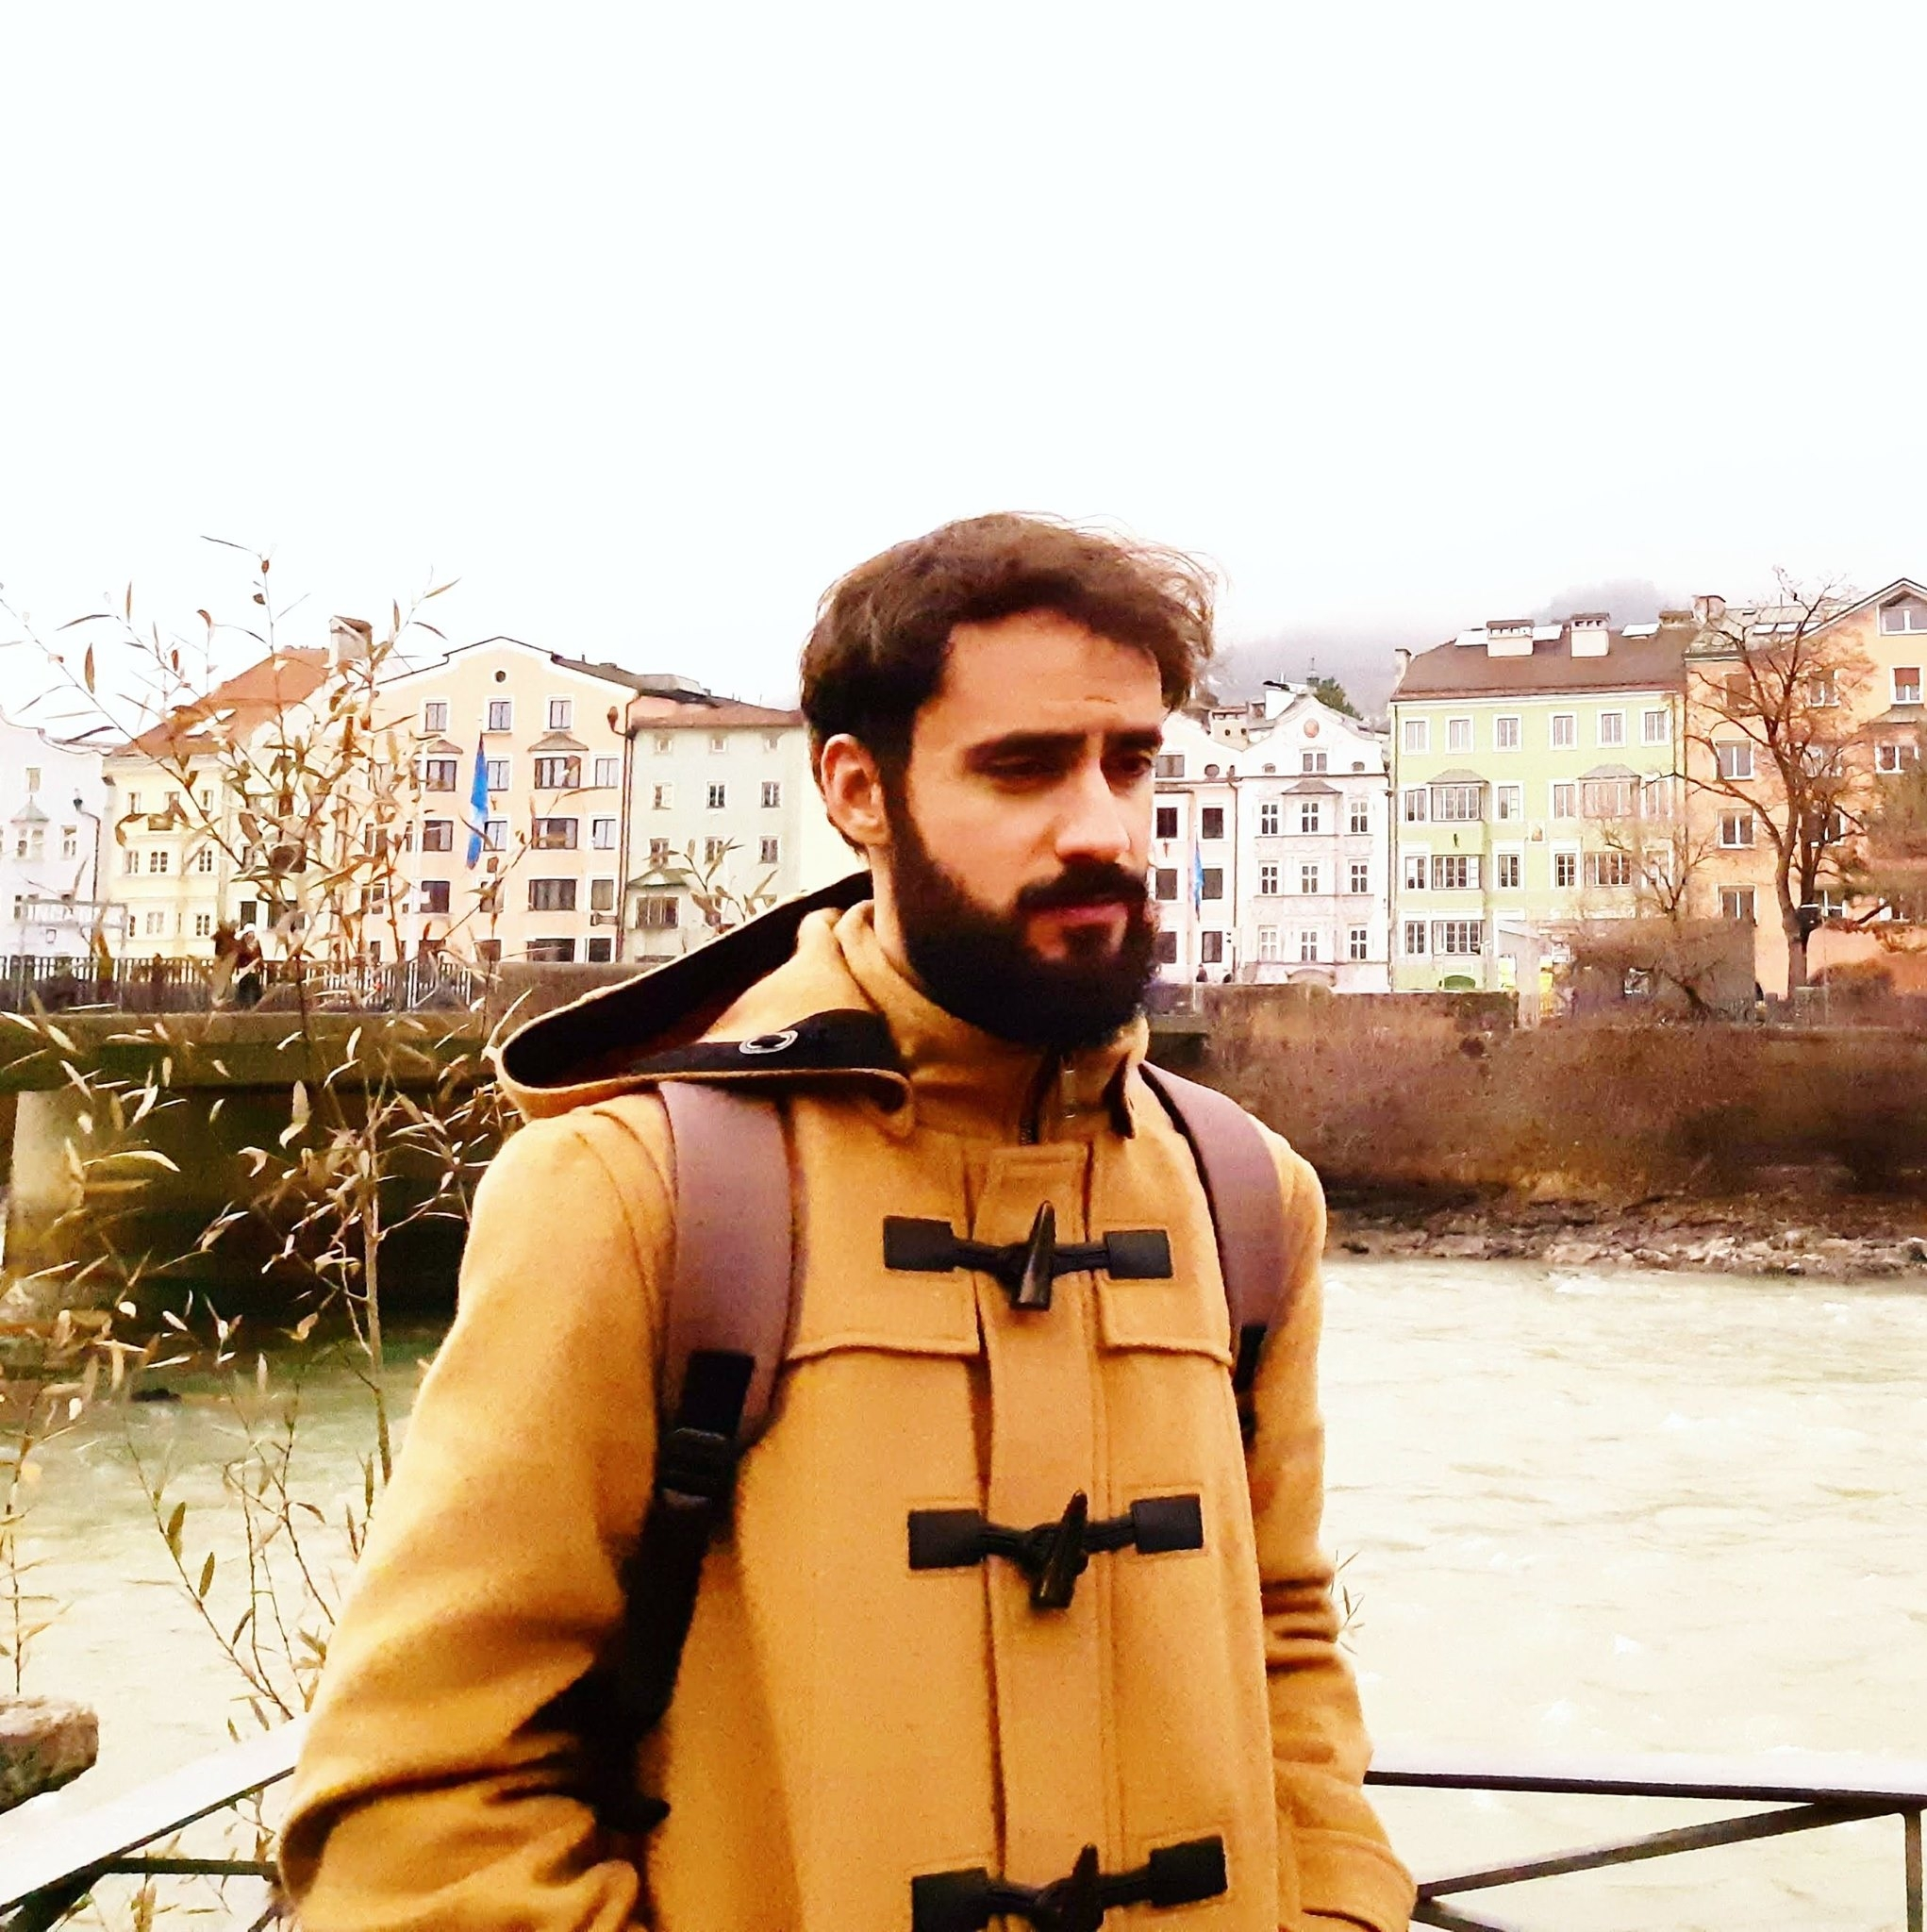
\includegraphics[width=3.5cm]{./figures/Paulo}
        \end{tabular}
         & \begin{tabular}{l}
               \parbox{0.6\linewidth}{%  change the parbox width as appropiate
                   \begin{itemize}
                    \item \textbf{Nome:} Paulo Victor da Fonseca \medskip
                    \item \textbf{Formação:} Doutorado em Economia - UFSC \medskip
                    \item \textbf{Áreas de pesquisa:} Macroeconomia. Políticas monetária e fiscal. Modelos DSGE. Modelos novo-Keynesianos com agentes heterogêneos. Modelos baseados em agentes. \medskip
                    \item \textbf{Website:} \href{https://pvfonseca.github.io}{pvfonseca.github.io} \medskip
                    \item \textbf{Contato:} \href{mailto:paulo.fonseca@udesc.br}{paulo.fonseca@udesc.br}
                \end{itemize}
               }
           \end{tabular} \\
    \end{tabular}
\end{frame}

\section{Motivação}
\begin{frame}{Escopo da Macroeconomia}
    \begin{itemize}
        \item Microeconomia: objeto de interesse é o comportamento individual (ou de um pequeno número) de firmas ou consumidores. \bigskip
        \item Macroeconomia: objeto de interesse é a economia como um todo.\medskip
        \begin{itemize}
            \item Comportamento agregado de firmas e consumidores. \medskip
            \item Comportamento dos governos. \medskip
            \item Nível agregado de atividade econômica de países individuais. \medskip
            \item Interações econômicas entre nações. \medskip
            \item Efeitos de políticas fiscal e monetária.
        \end{itemize}
    \end{itemize}
\end{frame}

\begin{frame}{Escopo da Macroeconomia}
    \begin{itemize}
        \item 1970s: redução da distinção entre teorias macro e micro. \bigskip
        \item \tikz[tstyle]{\node[nstyle](node1){Microfundamentação da macro:}} \medskip
        \begin{itemize}
            \item Agentes otimizadores dadas preferências e tecnologia. \medskip
            \item Ações dos agentes são compatíveis entre si. \medskip
        \end{itemize}
        \item Esta abordagem requer:\medskip
        \begin{itemize}
            \item Que sejamos explícitos a respeito dos pressupostos. \medskip
            \item Modelos como abstrações.
        \end{itemize}
        \begin{tikzpicture}[tpstyle]
            \draw[pencil, very thick] ([yshift=-1pt]node1.south west) to ([yshift=-1pt]node1.south east);
        \end{tikzpicture}
    \end{itemize}
\end{frame}

\begin{frame}{Escopo da Macroeconomia}
    \begin{itemize}
        \item A característica distinta da macro está nas questões que foca: \bigskip
        \begin{itemize}
            \item \tikz[tstyle]{\node[nstyle](node1){Crescimento de longo prazo:}} aumentos de capacidade produtiva e padrão de vida médio dos cidadãos ao longo de um longo período de tempo. \bigskip
            \item \tikz[tstyle]{\node[nstyle](node2){Ciclos econômicos:}} movimentos de expansão ou retração no nível agregado de atividade econômica no curto prazo.            
        \end{itemize}
        \begin{tikzpicture}[tpstyle]
            \draw[pencil, very thick, brick] ([yshift=-1pt]node1.south west) to ([yshift=-1pt]node1.south east);
            \draw[pencil, very thick] ([yshift=-1pt]node2.south west) to ([yshift=-1pt]node2.south east);
        \end{tikzpicture}
    \end{itemize}
\end{frame}

\begin{frame}{Por que estudar Macroeconomia?}
    \begin{itemize}
        \item Autointeresse: agregados macroeconômicos afetam nossa vida cotidiana. \bigskip
        \item Alfabetização cultural: compreensão do nosso mundo. \bigskip
        \item Bem-estar comum: essencial para formuladores de política econômica no design de boas políticas. \bigskip
        \item Responsabilidade civil: essencial para compreendermos nossos políticos.
    \end{itemize}
\end{frame}

\begin{frame}{Crescimento de longo prazo}
    \begin{center}
        \begin{minipage}[b]{.58\textwidth}
            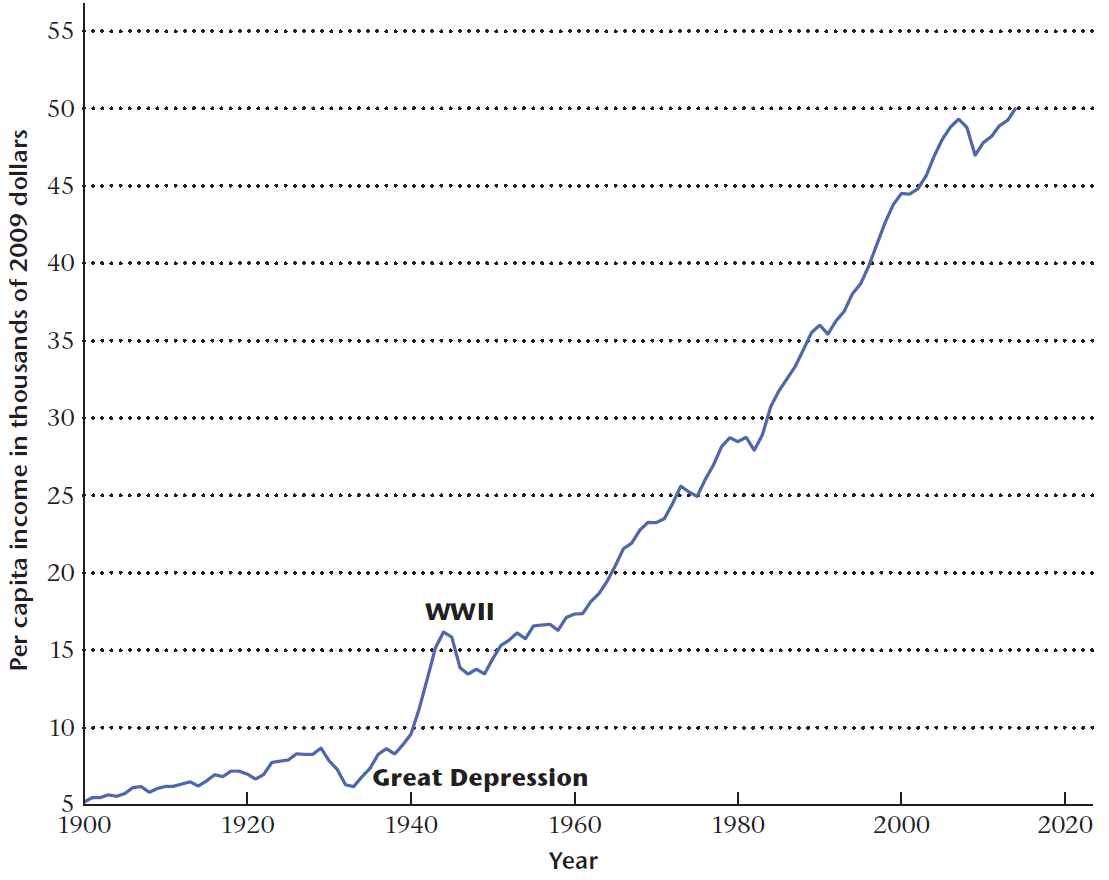
\includegraphics[width=\textwidth]{./figures/pib-usa.PNG}\\
            \tiny{{\scshape Fonte}: \ Williamson (2018).}
        \end{minipage}
    \end{center}
\end{frame}

\begin{frame}{Crescimento de longo prazo}
    \begin{center}
        \begin{minipage}[b]{0.9\textwidth}
            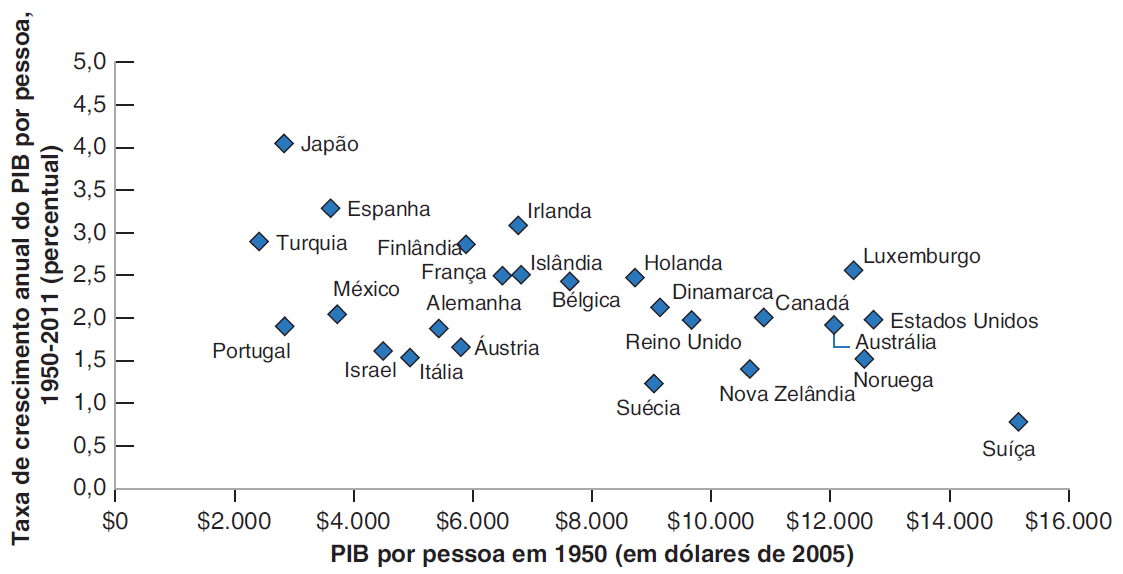
\includegraphics[width=\textwidth]{./figures/conv ocde.PNG}\\
            \tiny{{\scshape Fonte}: \ Blanchard (2017).}
        \end{minipage}
    \end{center}
\end{frame}

\begin{frame}{Crescimento de longo prazo}
    \begin{center}
        \begin{minipage}[b]{0.9\textwidth}
            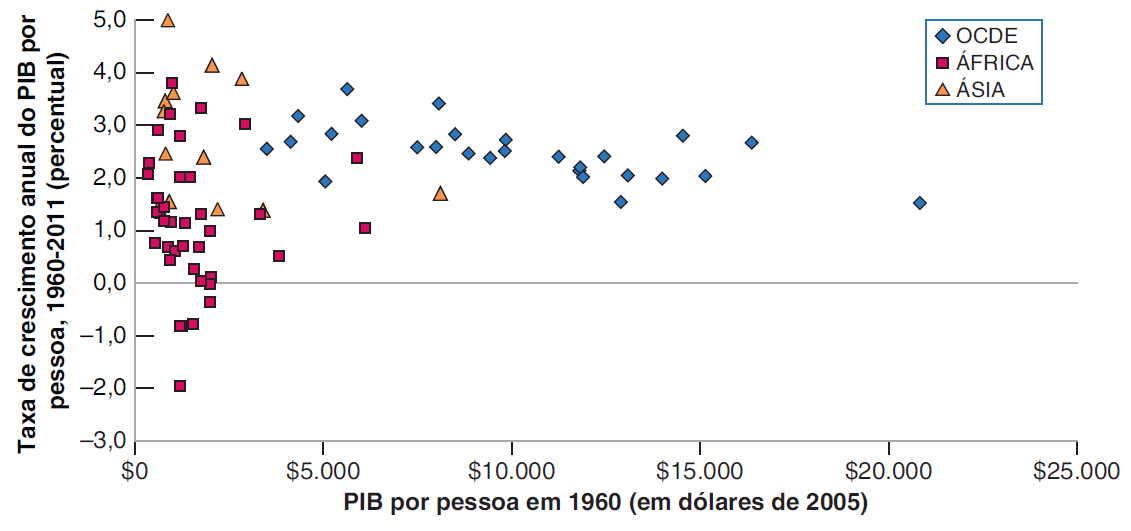
\includegraphics[width=\textwidth]{./figures/conv nocde.PNG}\\
            \tiny{{\scshape Fonte}: \ Blanchard (2017).}
        \end{minipage}
    \end{center}
\end{frame}

\begin{frame}{Por que nos preocupamos com PIB?}
    \begin{center}
        \begin{minipage}[b]{.7\textwidth}
            \href{https://ourworldindata.org/grapher/median-daily-per-capita-expenditure-vs-gdp-per-capita}{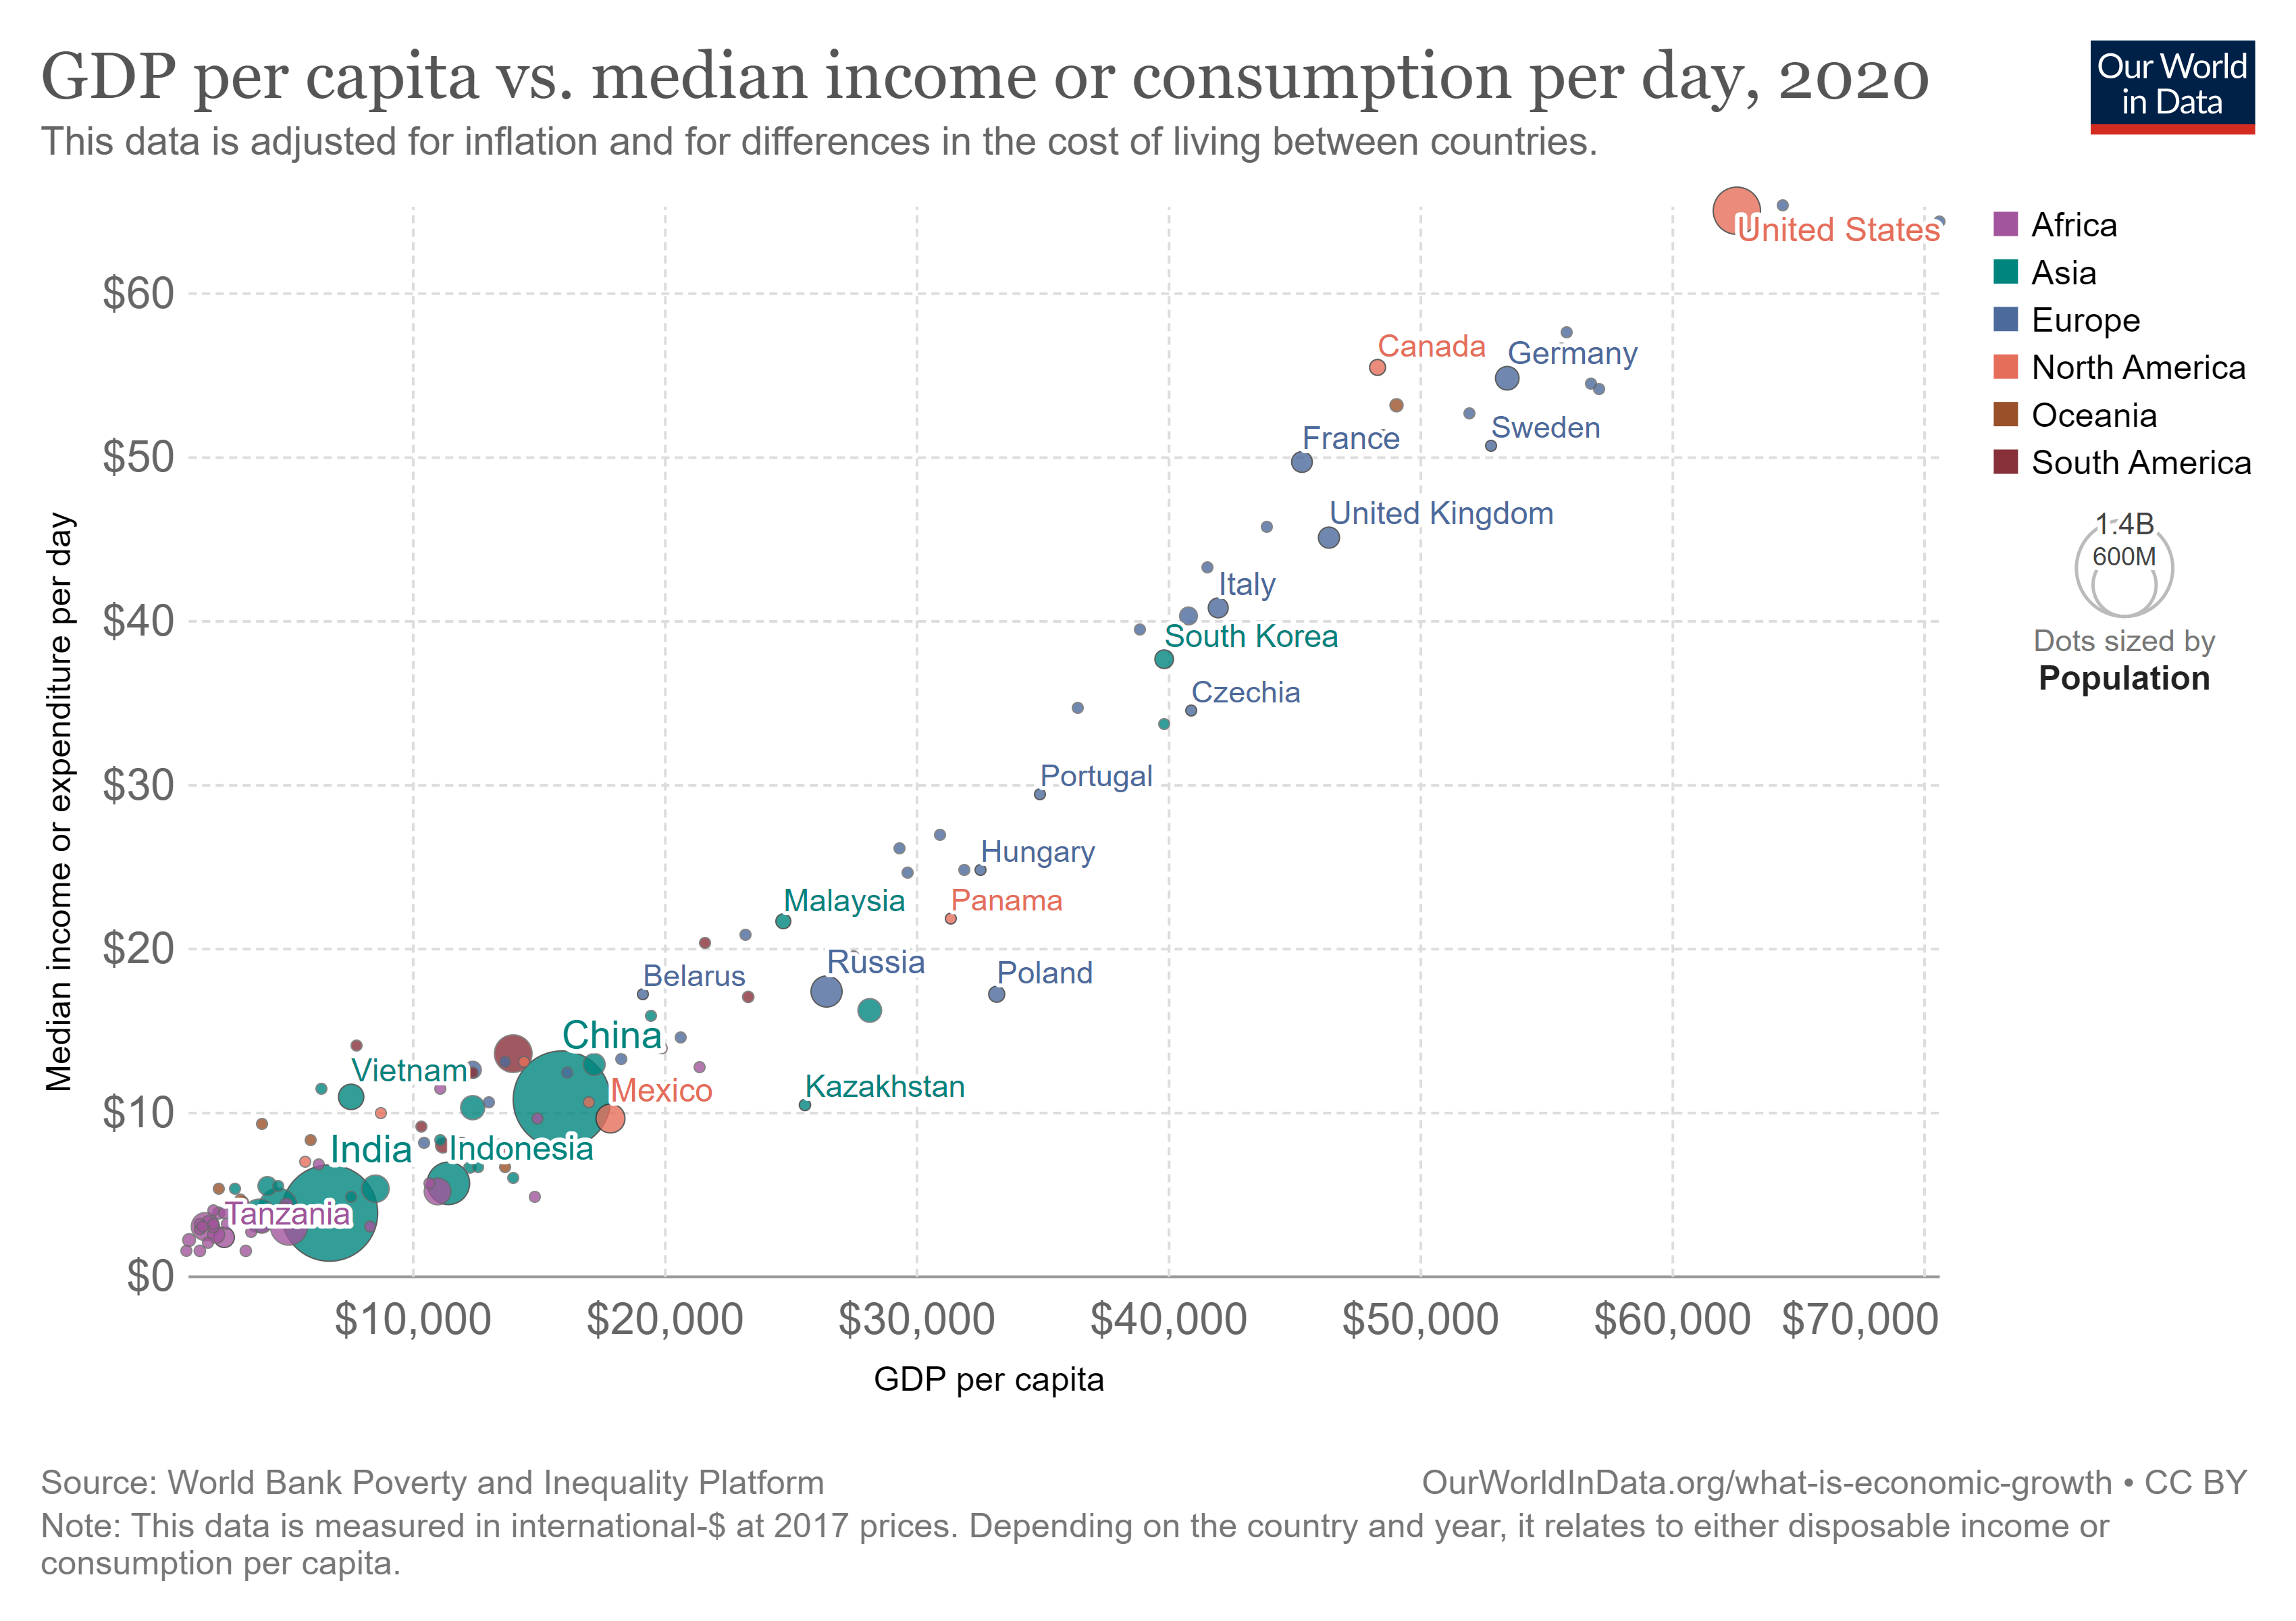
\includegraphics[width=\textwidth]{./figures/gdp x consumption.png}}
        \end{minipage}
    \end{center}
\end{frame}

\begin{frame}{Por que nos preocupamos com PIB?}
    \begin{center}
        \begin{minipage}[b]{.7\textwidth}
            \href{https://ourworldindata.org/grapher/life-expectancy-vs-gdp-per-capita}{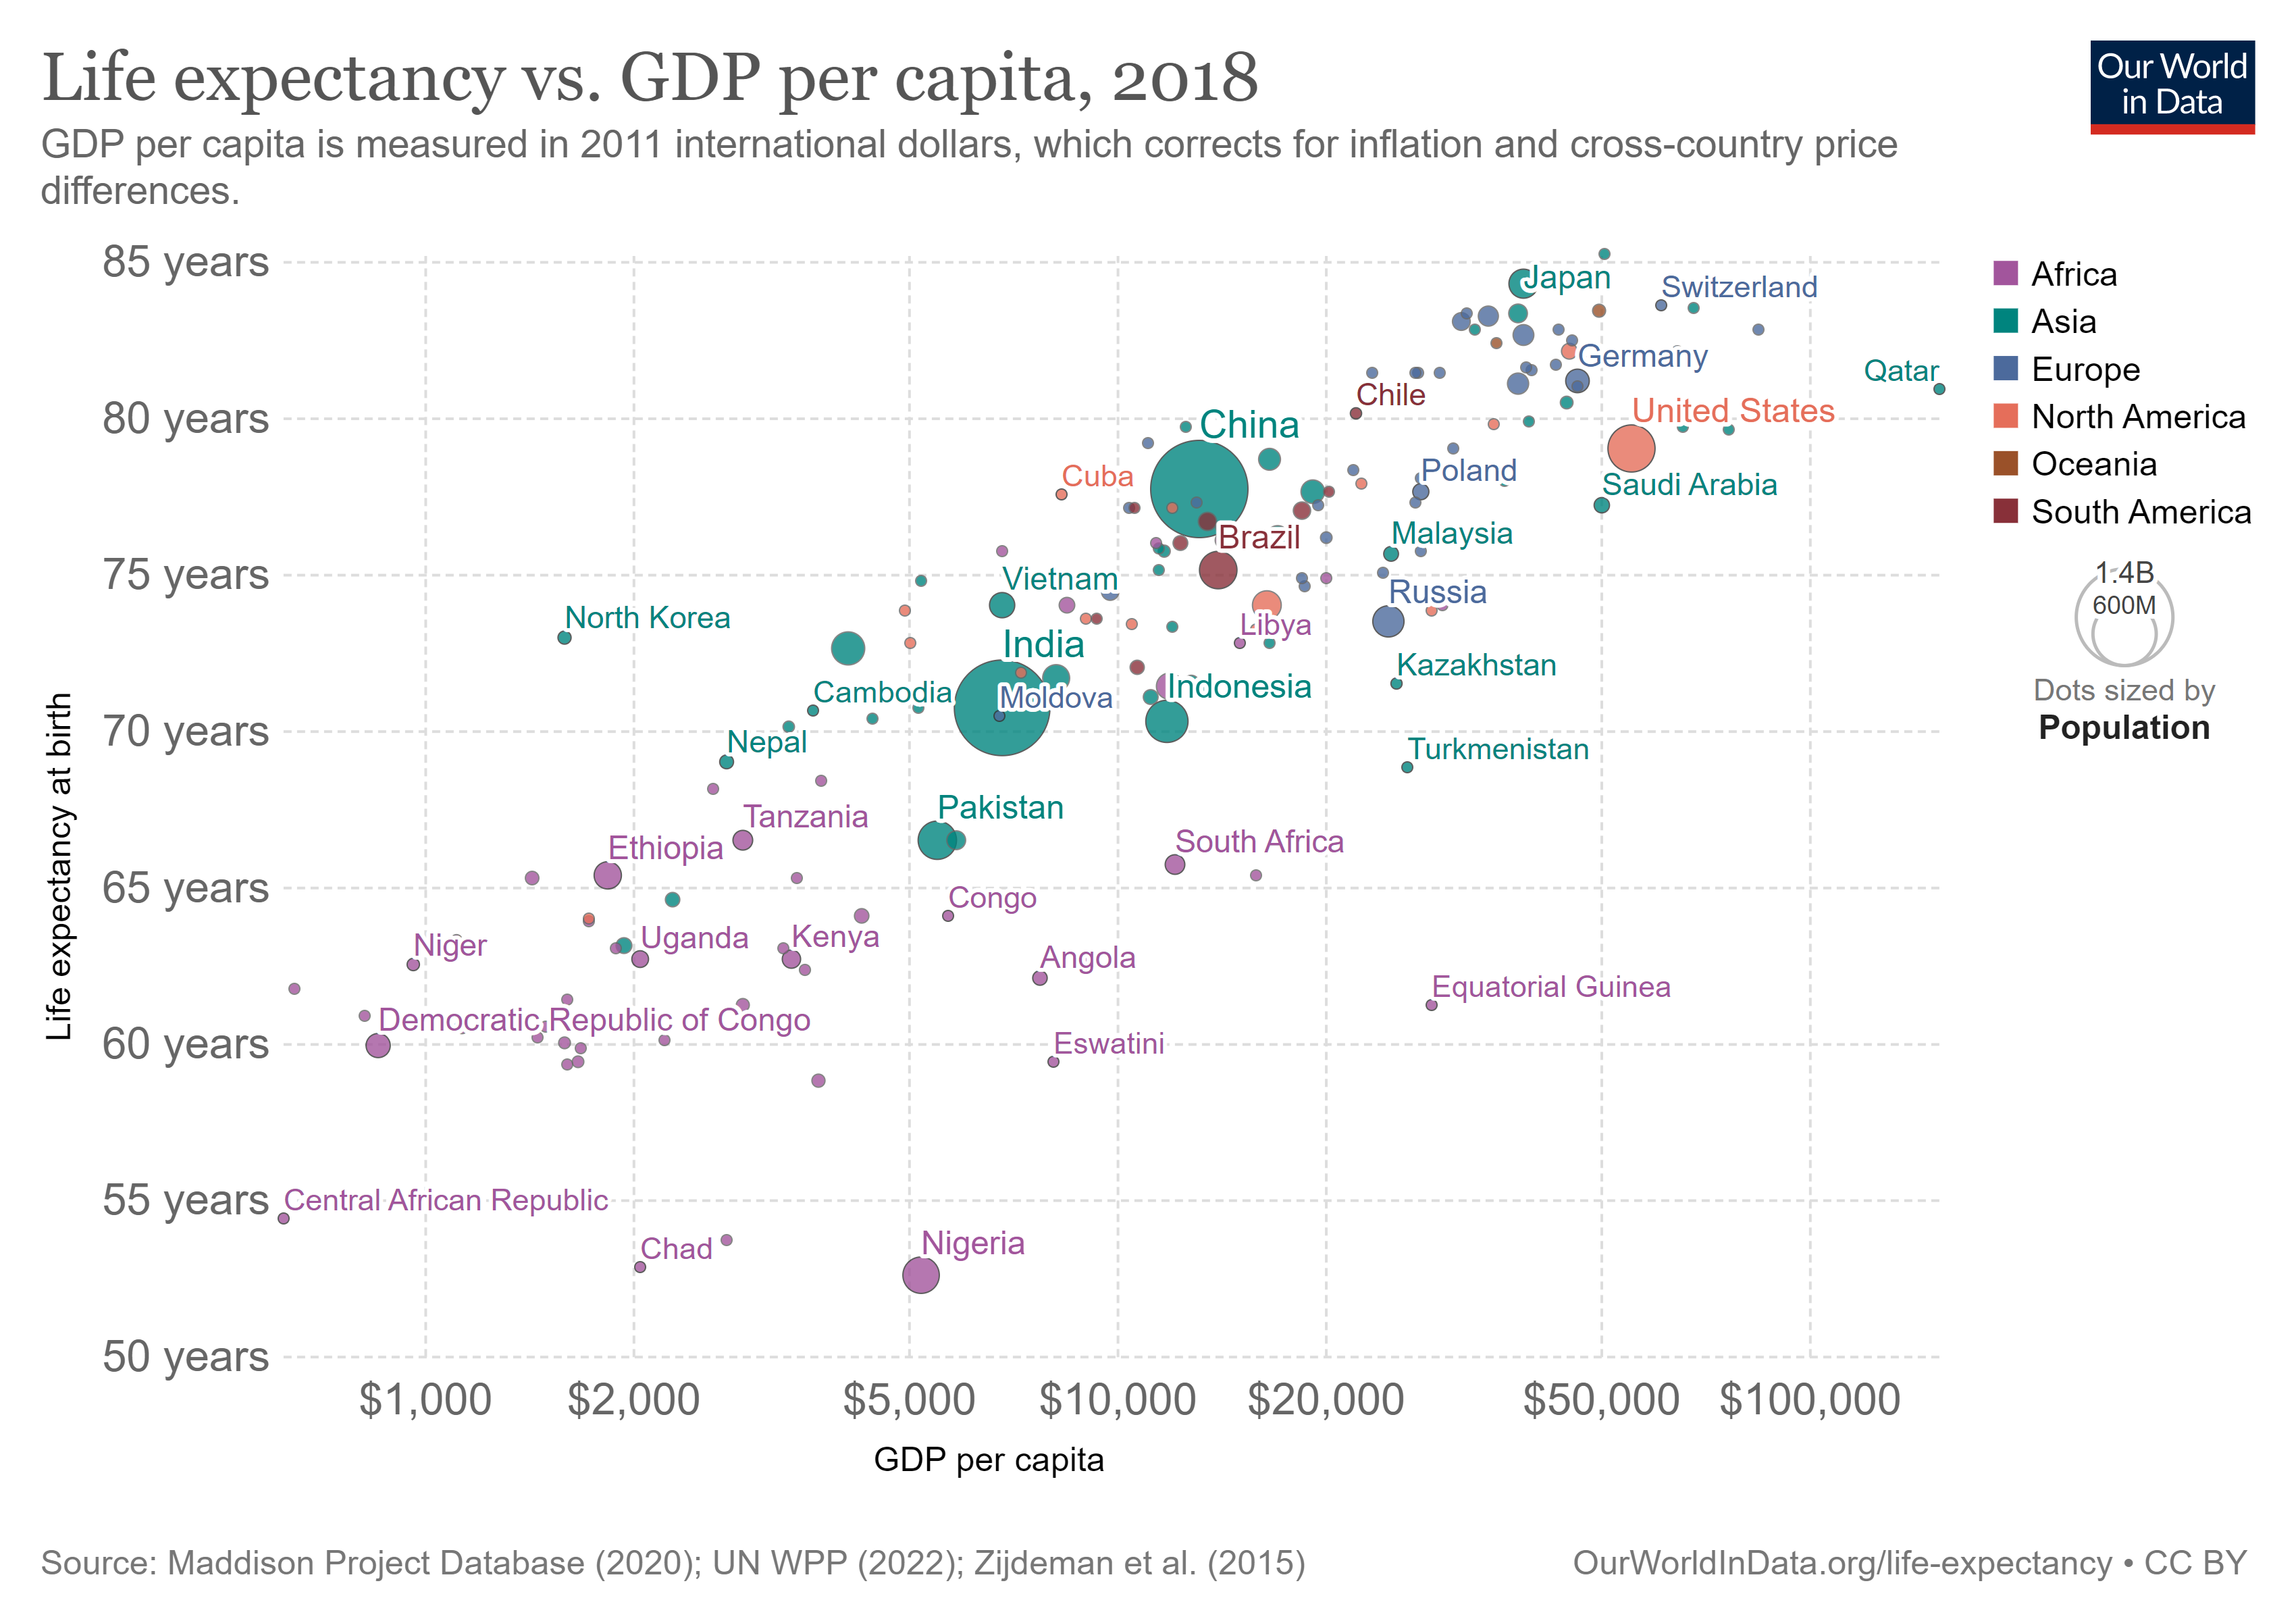
\includegraphics[width=\textwidth]{./figures/life exp x gdp.png}}
        \end{minipage}
    \end{center}
\end{frame}

\begin{frame}{Por que nos preocupamos com PIB?}
    \begin{center}
        \begin{minipage}[b]{.7\textwidth}
            \href{https://www.nytimes.com/2008/04/16/business/16leonhardt.html}{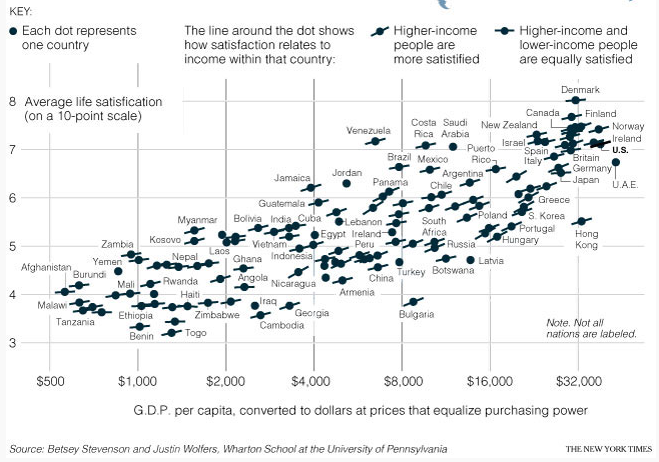
\includegraphics[width=\textwidth]{./figures/gdp x satisfaction.PNG}}
        \end{minipage}
    \end{center}
\end{frame}

\begin{frame}{Ciclos econômicos}
    \begin{center}
        \begin{minipage}[b]{.6\textwidth}
            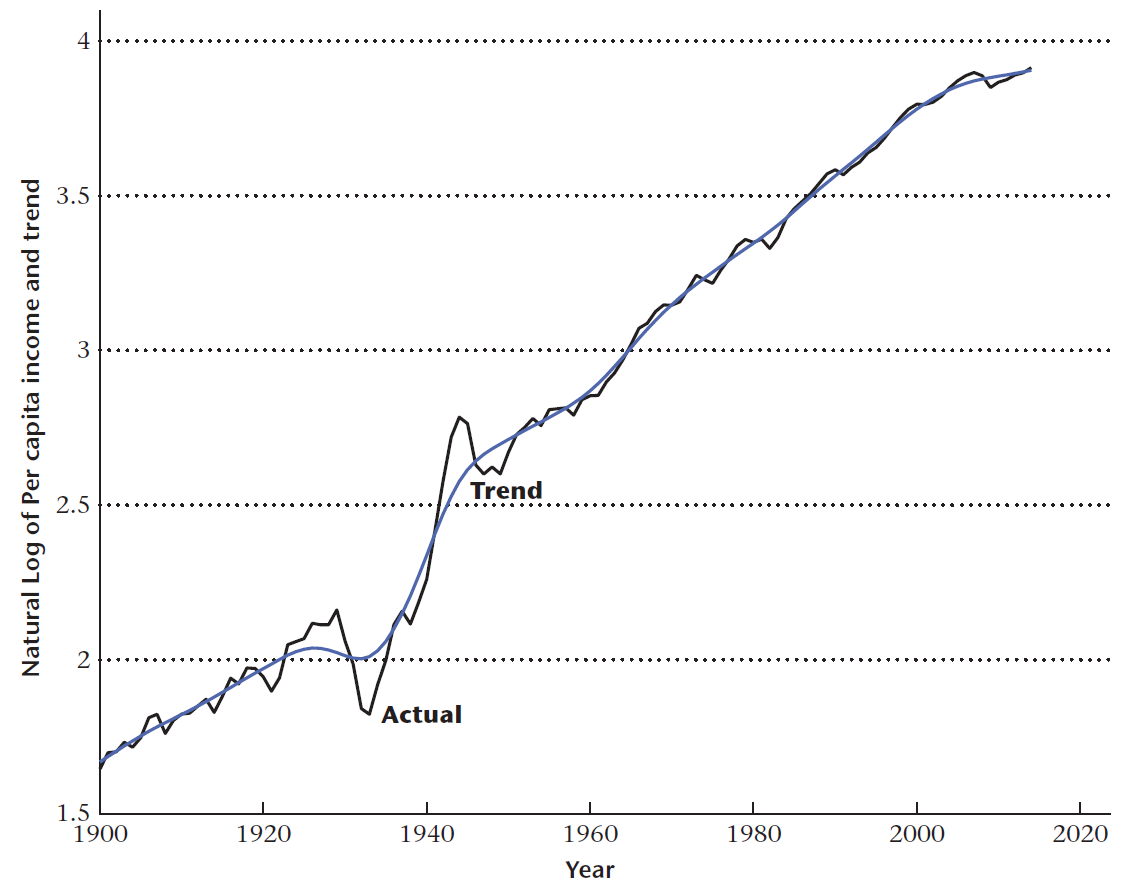
\includegraphics[width=\textwidth]{./figures/gdp decomp.PNG}
            \tiny{{\scshape Fonte}: \ Williamson (2018).}
        \end{minipage}
    \end{center}
\end{frame}

\begin{frame}{Ciclos econômicos}
    \begin{center}
        \begin{minipage}[b]{.58\textwidth}
            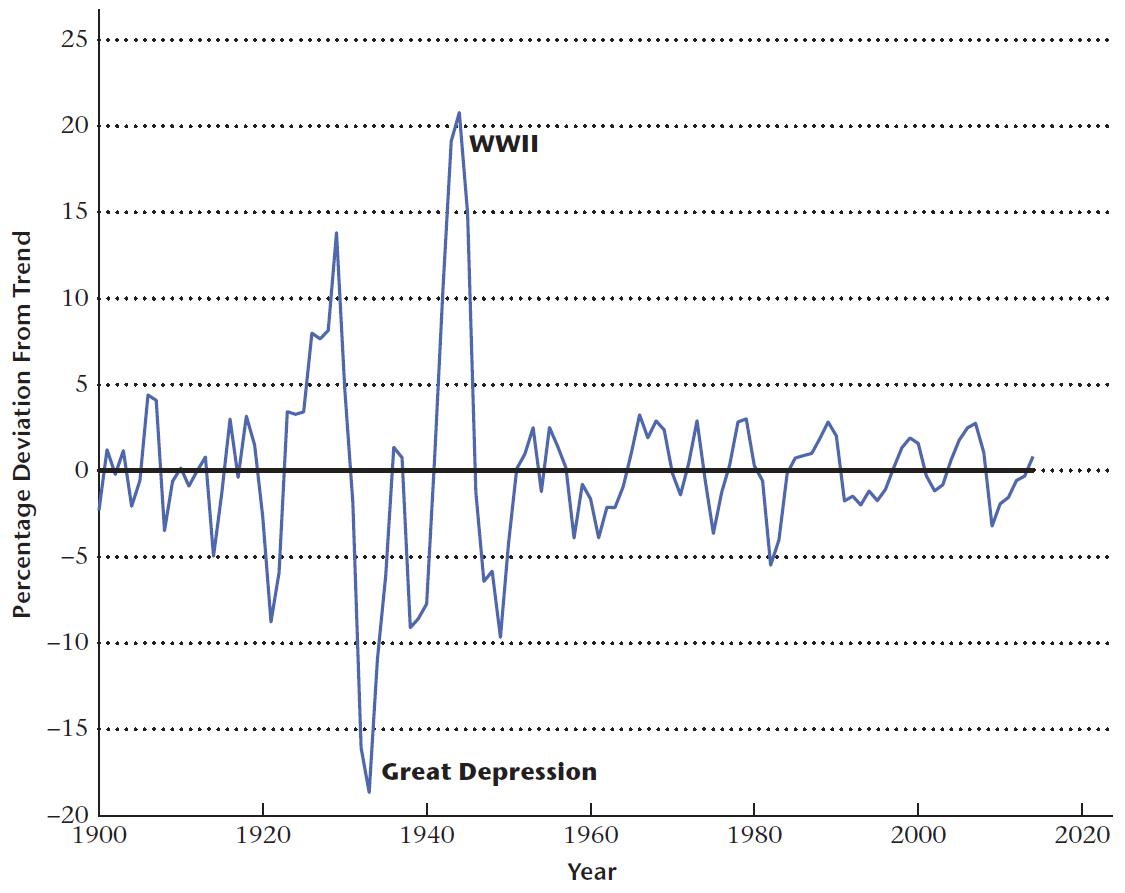
\includegraphics[width=\textwidth]{./figures/ciclo.PNG}
            \tiny{{\scshape Fonte}: \ Williamson (2018).}
        \end{minipage}
    \end{center}
\end{frame}

\begin{frame}{Desemprego}
    \begin{center}
        \begin{minipage}[b]{.57\textwidth}
            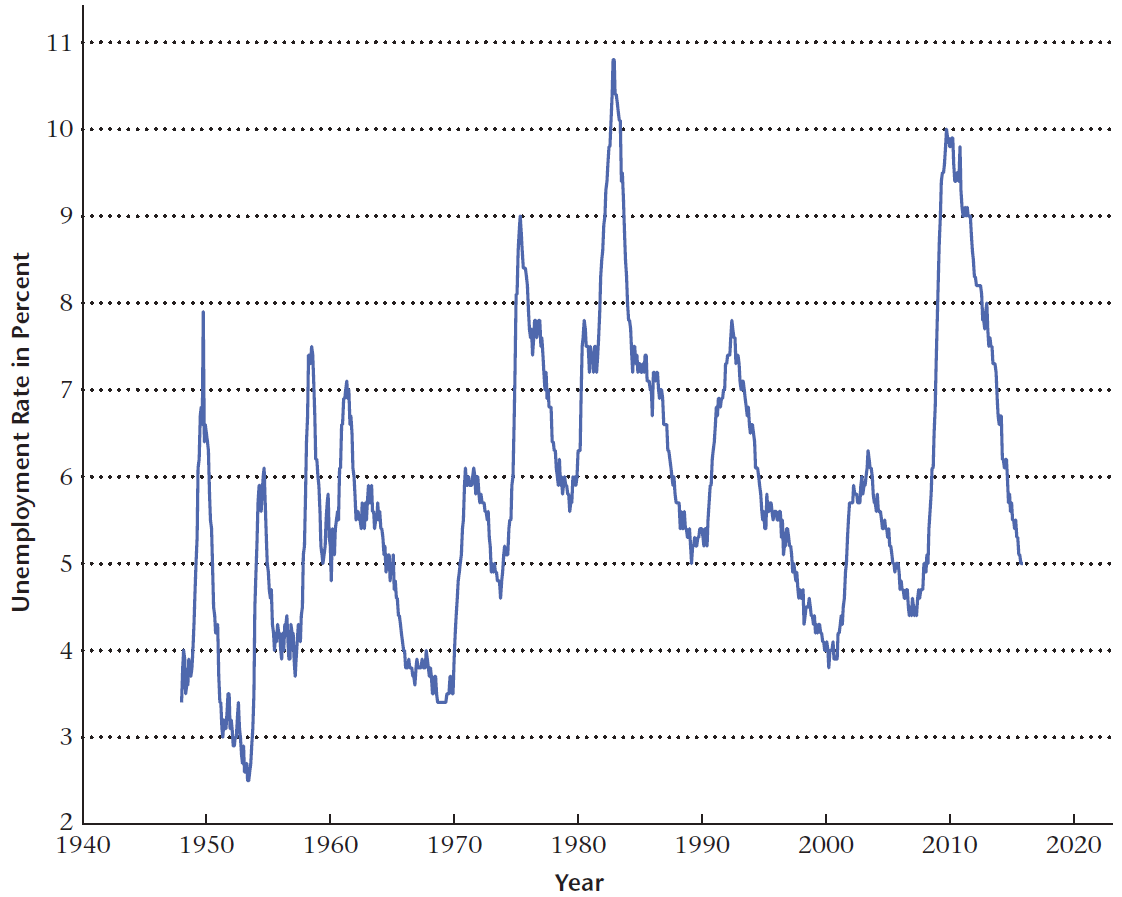
\includegraphics[width=\textwidth]{./figures/unemployment.PNG}
            \tiny{{\scshape Fonte}: \ Williamson (2018).}
        \end{minipage}
    \end{center}
\end{frame}

\begin{frame}{Por que nos preocupamos com desemprego?}
    \begin{itemize}
        \item Desemprego baixo ou alto é um sintoma de ineficiência.\medskip
        \begin{itemize}
            \item Desemprego elevado: muitos recursos ociosos.\medskip
            \item Desemprego baixo: escassez de mão-de-obra, muitos recursos despendidos no recrutamento de trabalhadores.\bigskip
        \end{itemize}
        \item Efeito direto sobre bem-estar: desemprego reduz bem-estar do desempregado (especialmente aqueles desempregados por mais tempo).\medskip
        \begin{itemize}
            \item Baixa saúde física e mental (ansiedade, baixa auto-estima, baixa satisfação com a vida), mesmo após controlarmos para a renda.
        \end{itemize}
    \end{itemize}
\end{frame}

\begin{frame}{Por que nos preocupamos com desemprego?}
    \begin{tabular}{cl}
        \begin{tabular}{c}
            \href{https://news.gallup.com/poll/171044/depression-rates-higher-among-long-term-unemployed.aspx}{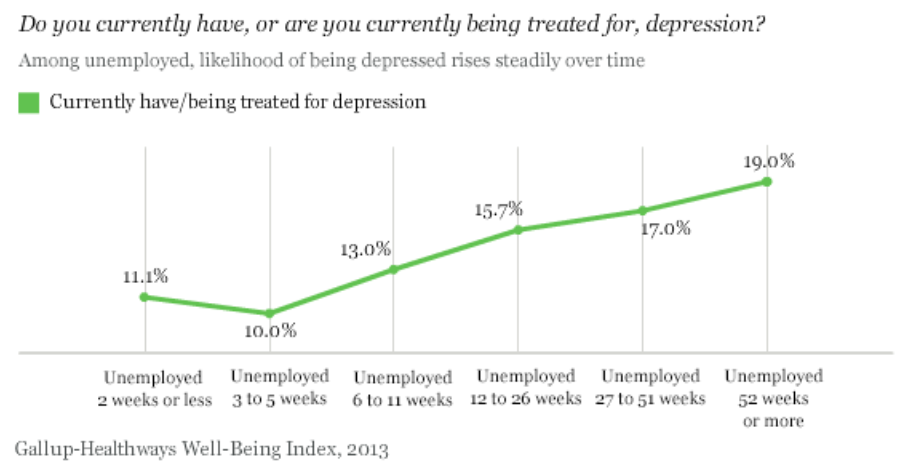
\includegraphics[width=.5\textwidth]{./figures/depression.PNG}}
        \end{tabular}
         & \begin{tabular}{c}
            \href{https://news.gallup.com/poll/171044/depression-rates-higher-among-long-term-unemployed.aspx}{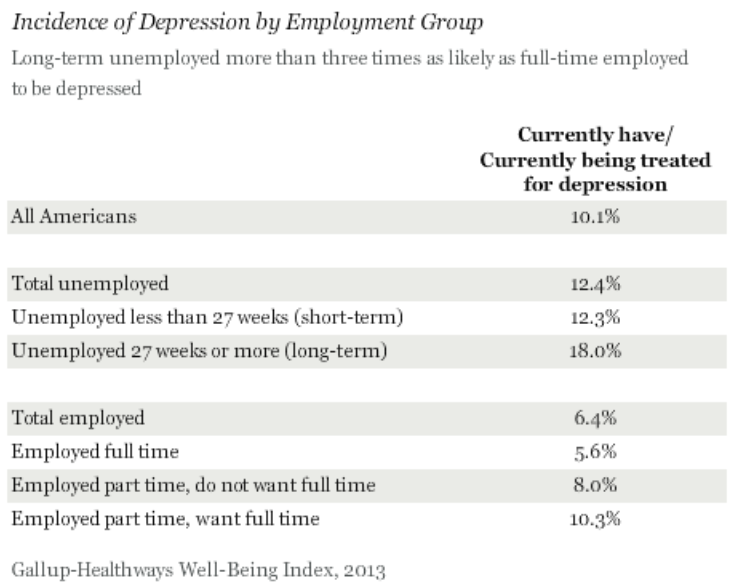
\includegraphics[width=.4\textwidth]{./figures/depression table.PNG}}
           \end{tabular} \\
    \end{tabular}
\end{frame}

\begin{frame}{Por que nos preocupamos com desemprego?}
    \begin{center}
        \begin{minipage}[b]{.57\textwidth}
            \href{https://wol.iza.org/articles/unemployment-and-happiness/long}{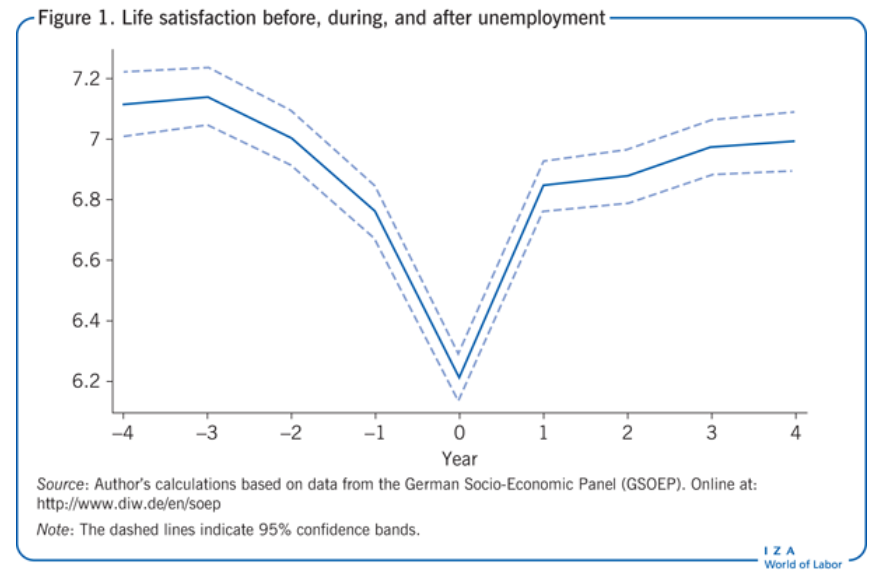
\includegraphics[width=\textwidth]{./figures/satisfaction.PNG}}            
        \end{minipage}
    \end{center}
\end{frame}

\begin{frame}{Inflação}
    \begin{center}
        \begin{minipage}[b]{\textwidth}
            \begin{tikzpicture}
                \node[inner sep=0] (image) at (0,0){\href{https://fred.stlouisfed.org/series/CPIAUCSL}{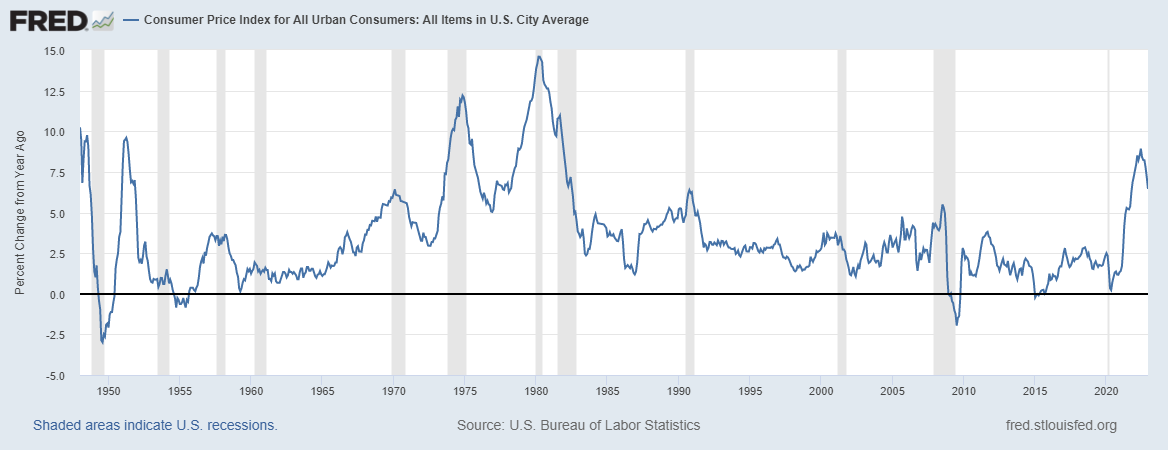
\includegraphics[width=\textwidth]{./figures/inflation.png}}};
                \draw[arrow,->,opacity=1,brick] (4,0.4) to[bend right] +(-0.1,+0.9) node[anchor=east,opacity=1,brick] {\normalsize{\hand - Grande Moderação}};
                \node[rectangle, fill=gold,opacity=0.2,rounded corners=.1cm, minimum width=4.3cm,minimum height=4.35cm] at (2.5,0.15) {};
            \end{tikzpicture}                        
        \end{minipage}
    \end{center}
\end{frame}

\begin{frame}{Por nos importamos com inflação?}
    \begin{itemize}
        \item Nem todos os preços/salários aumentam proporcionalmente. Inflação afeta poder de compra de diferentes agentes de maneira distinta, afeta distribuição de renda.\medskip
        \begin{itemize}
            \item Alguns preços e salários são fixos por lei (e.g., salário mínimo nos EUA).        
        \begin{center}
            \begin{minipage}[b]{.8\textwidth}
                \href{https://fred.stlouisfed.org/series/FEDMINNFRWG}{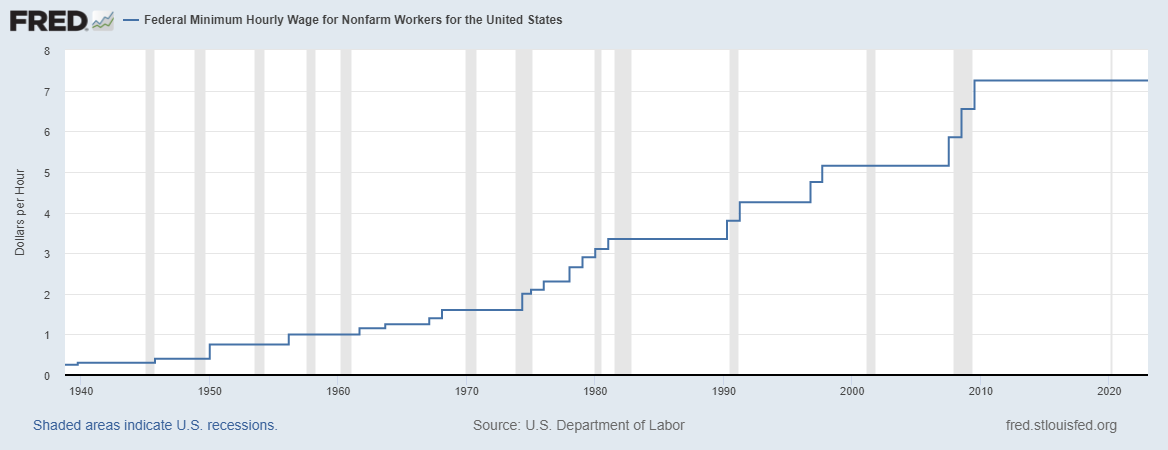
\includegraphics[width=\textwidth]{./figures/minimum wage.png}}            
            \end{minipage}
        \end{center}
    \item Alguns preços e salários são fixados por contratos de longo prazo (e.g., alguns pagamentos de empréstimo ou pensões).
    \end{itemize}
    \end{itemize}
\end{frame}

\begin{frame}{Por nos importamos com inflação?}
    \begin{itemize}
        \item Inflação pode distorcer o sistema tributário.
        \begin{center}
            \begin{minipage}[b]{.5\textwidth}
                \href{https://oglobo.globo.com/economia/imposto-de-renda/noticia/2023/01/imposto-de-renda-defasagem-na-tabela-atinge-148percent-e-chega-a-recorde-historico.ghtml}{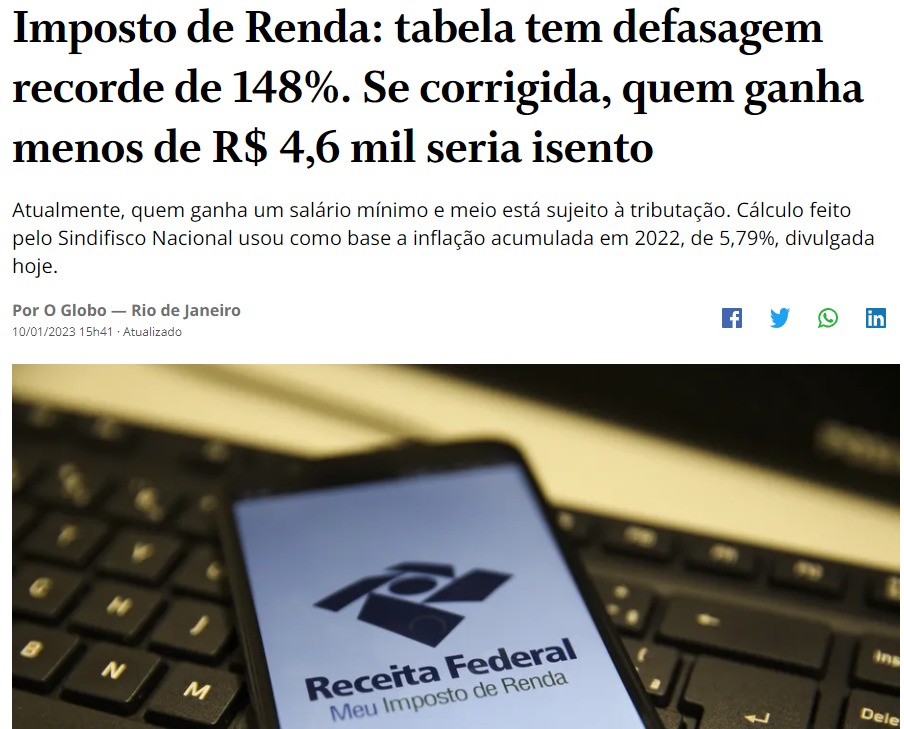
\includegraphics[width=\textwidth]{./figures/irf.PNG}}
            \end{minipage}
        \end{center}
        \item Inflação causa \textcolor{purple}{incerteza}.
    \end{itemize}
\end{frame}

\begin{frame}{Lei de Okun}
    \begin{center}
        \begin{minipage}[b]{.7\textwidth}
            \href{https://en.wikipedia.org/wiki/Okun's_law}{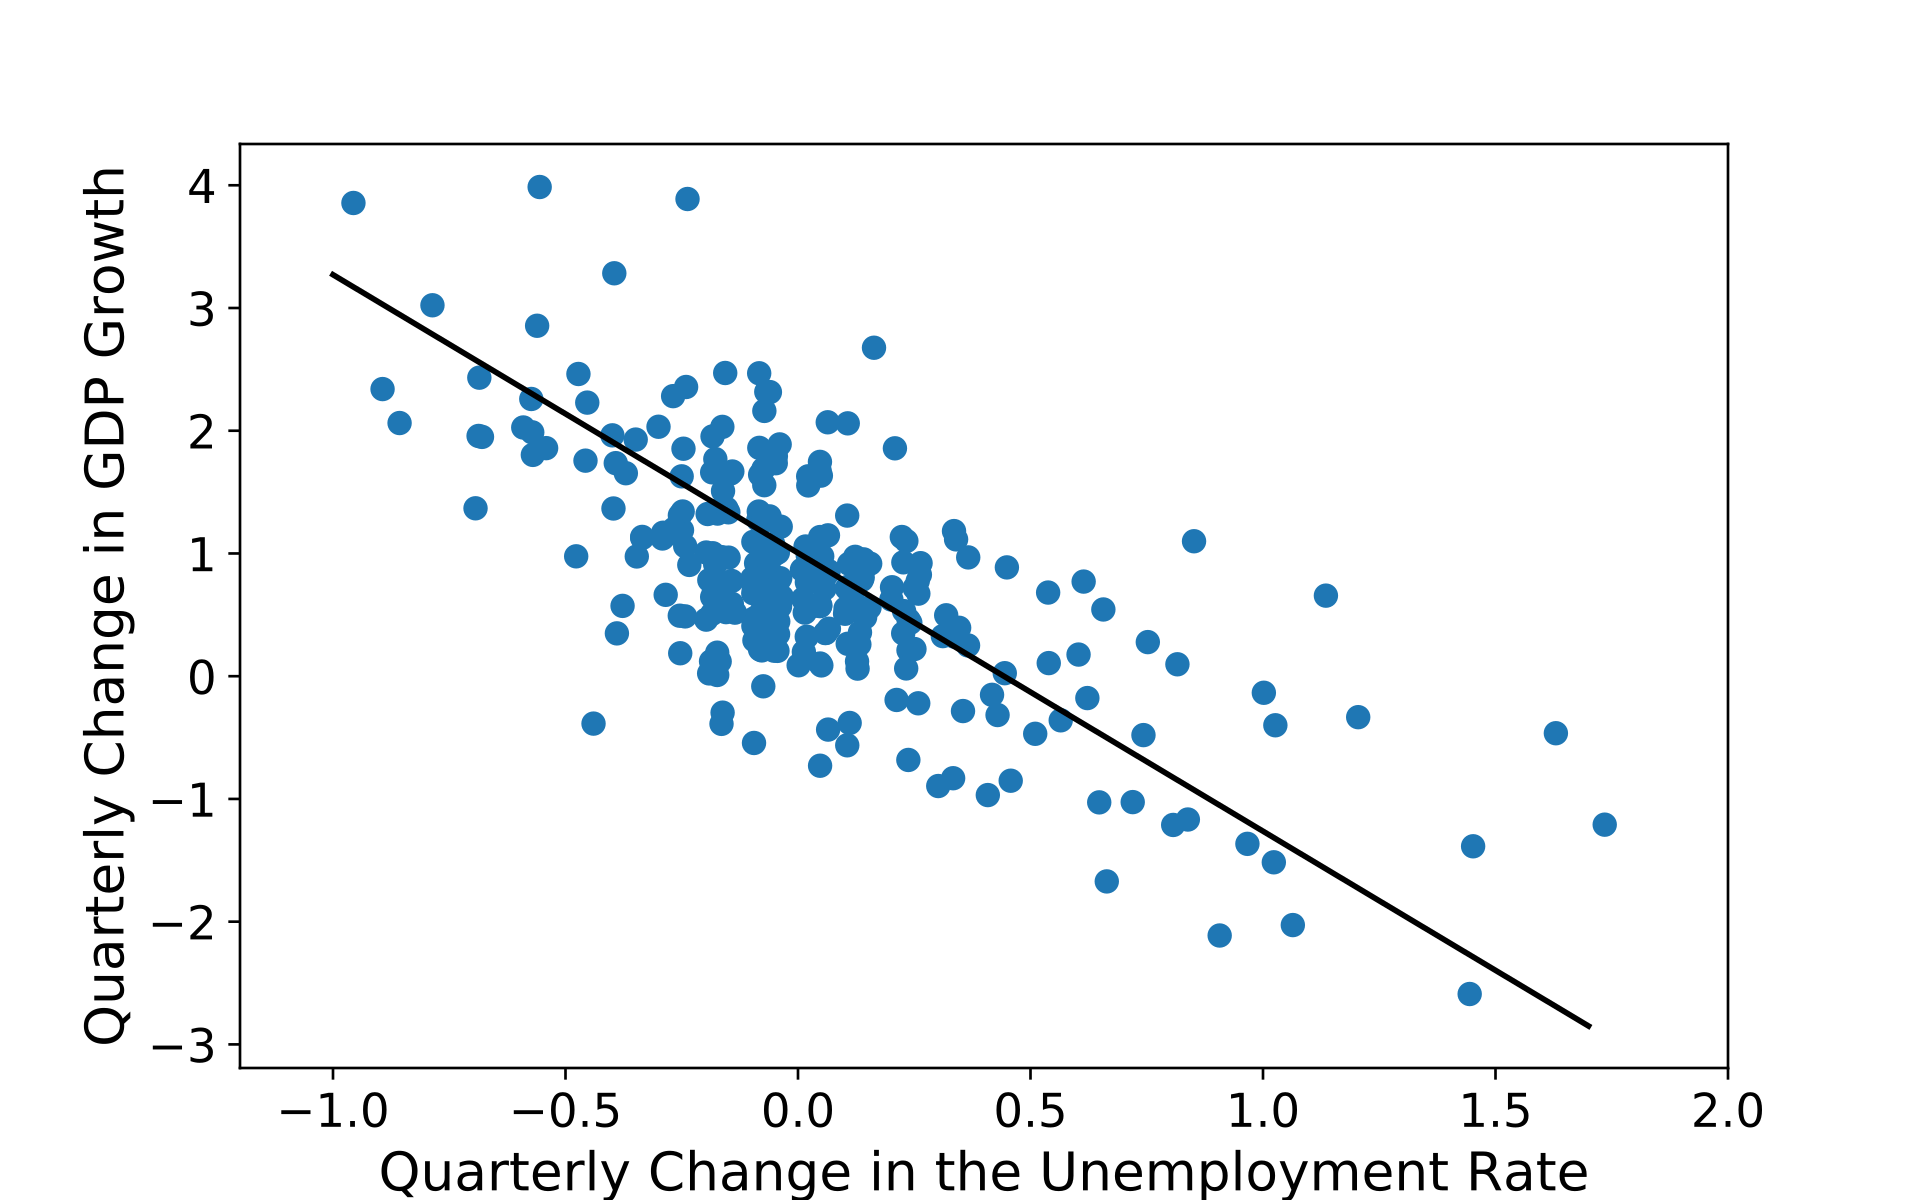
\includegraphics[width=\textwidth]{./figures/okun law.png}}
            \tiny{{\scshape Lei de Okun}: \ Estados Unidos (1948-2016).}
        \end{minipage}
    \end{center}
\end{frame}

\begin{frame}{Curva de Phillips}
    \begin{center}
        \begin{minipage}[b]{.65\textwidth}
            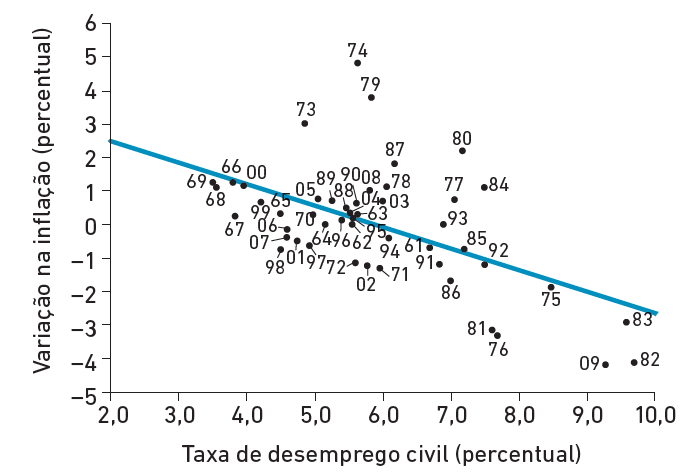
\includegraphics[width=\textwidth]{./figures/phillips.PNG}
            \tiny{{\scshape Fonte}: \ Dornbusch, Fischer e Startz (2013).}
        \end{minipage}
    \end{center}
\end{frame}

\begin{frame}
    {Controvérsias entre macroeconomistas}
    \begin{itemize}
        \item A maioria dos pesquisadores em macro concordam em um amplo conjunto de questões.\bigskip
        \item Há um amplo consenso em teoria do crescimento.\bigskip
        \item Em teoria dos ciclo econômicos, o consenso é menor.\bigskip
        \item Questões normativas: papel do governo na estabilização.
    \end{itemize}
\end{frame}

\begin{frame}{Macroeconomia I}
    \begin{itemize}
        \item  Mas o que determina o nível do produto agregado em uma economia?\bigskip
              \begin{itemize}
                  \item \tikz[tstyle]{\node[nstyle](node2){Curto prazo.}} Variações ano a ano no produto decorrem principalmente de movimentos na demanda agregada. Mudanças na demanda (e.g., confiança do consumidor, taxas de juros) podem levar a uma diminuição no produto (recessão) ou a um aumento no PIB (expansão).\medskip
                        \begin{tikzpicture}[tpstyle]
                            \draw[pencil, very thick] ([yshift=-1pt]node2.south west) to ([yshift=-1pt]node2.south east);
                        \end{tikzpicture}

                  \item \tikz[tstyle]{\node[nstyle](node2){Médio prazo.}} Economia tende a voltar ao nível de produto determinado por fatores de oferta: estoque de capital, nível de tecnologia e tamanho da força de trabalho. Ao longo de uma década, esses fatores variam em um ritmo lento o suficiente a ponto de podermos tomá-los como dados.\medskip
                        \begin{tikzpicture}[tpstyle]
                            \draw[pencil, very thick] ([yshift=-1pt]node2.south west) to ([yshift=-1pt]node2.south east);
                        \end{tikzpicture}

                  \item \tikz[tstyle]{\node[nstyle](node2){Longo prazo.}} Para entender o crescimento sustentado ao longo de décadas (e.g., por que o capital e o nível de tecnologia chinesas cresceram tanto desde 1980?) examinamos fatores como sistema educacional, taxa de poupança e o papel do governo e instituições.
                        \begin{tikzpicture}[tpstyle]
                            \draw[pencil, very thick, brick] ([yshift=-1pt]node2.south west) to ([yshift=-1pt]node2.south east);
                        \end{tikzpicture}
              \end{itemize}
    \end{itemize}
\end{frame}

\begin{frame}{Macroeconomia I}
    A disciplina 33MAC1 - Macroeconomia I foca nos determinantes do produto agregado de equilíbrio em uma \tikz[tstyle]{\node[nstyle](node0){economia fechada}} \begin{tikzpicture}[tpstyle]
        \node[pencil,draw, minimum height=0.5cm, minimum width=3cm] (box0) at (node0) {};
    \end{tikzpicture} tanto no \tikz[tstyle]{\node[nstyle](node2){curto}} \begin{tikzpicture}[tpstyle]
        \draw[pencil, very thick] ([yshift=-1pt]node2.south west) to ([yshift=-1pt]node2.south east);
    \end{tikzpicture} quanto no \tikz[tstyle]{\node[nstyle](node2){médio}} prazo. O curso é dividido em cinco blocos:\bigskip
    \begin{tikzpicture}[tpstyle]
        \draw[pencil, very thick] ([yshift=-1pt]node2.south west) to ([yshift=-1pt]node2.south east);
    \end{tikzpicture}
    \begin{enumerate}
        \item Introdução e modelo clássico\medskip
        \item Demanda agregada e curva IS\medskip
        \item Oferta agregada (médio prazo)\medskip
        \item Modelo de 3 equações e política macroeconômica\medskip
        \item Políticas macroeconômicas \tikz[tstyle]{\node[nstyle](node1){convencionais}}
              \begin{tikzpicture}[tpstyle]
                  \draw[arrow,->,brick,opacity=0.5] ([yshift=-2pt]node1.south) to[bend right] +(1.6,-0.2) node[anchor=west] {\hand Sujeito a disponibilidade de tempo.};
              \end{tikzpicture}
    \end{enumerate}
\end{frame}

\section{Ementa}
\begin{frame}{Macroeconomia I: Ementa}
    \begin{center}
        \begin{minipage}{.9\textwidth}
            \NB{Agregados econômicos. Determinação do produto no modelo clássico: mercado de trabalho e curva de oferta agregada. Poupança, investimento e taxa de juros de equilíbrio. Teoria quantitativa da moeda e demanda agregada. Produto de equilíbrio no modelo keynesiano. Mercado de trabalho. Modelo de demanda e oferta agregadas. Curva de Phillips aumentada.
            }
        \end{minipage}
    \end{center}

\end{frame}

\section{Objetivo}
\begin{frame}{Macroeconomia I: objetivo}
    \begin{center}
        \begin{minipage}{.9\textwidth}
            \NB{Apresentar os princípios básicos da teoria macroeconômica e seus diversos domínios de aplicação.
                \bigskip
                O curso se propõe a familiarizar o estudante com os principais modelos macroeconômicos para determinação do produto de equilíbrio a partir da metodologia de equilíbrio geral, onde são tratadas as interações entre vários mercados, bem como os efeitos da ação do governo, em nível agregado. Isso permitirá o conhecimento dos instrumentos de análise e prescrição de políticas macroeconômicas.}
        \end{minipage}
    \end{center}
\end{frame}

\section{Formato das aulas e avaliações}
\begin{frame}{Formato das aulas e sistema de avaliação}
    \begin{itemize}
        \item A disciplina apoia-se, fundamentalmente, em livros-texto e notas de aula e será ministrada por meio de aulas expositivas.\bigskip

        \item As aulas acontecerão às:\medskip
              \begin{itemize}
                  \item Terças-feiras das 10:15 às 11:55
                  \item Quintas-feiras das 08:20 às 10:00\bigskip
              \end{itemize}

        \item A avaliação será realizada a partir dos procedimentos abaixo:\medskip
              \begin{itemize}
                  \item Atividade avaliativa I (PI): 30\%
                  \item Atividade avaliativa II (PII): 30\%
                  \item Atividade avaliativa III (PIII): 30\%
                  \item Trabalhos adicionais: 10\%
              \end{itemize}
    \end{itemize}
\end{frame}

\begin{frame}{Formato das aulas e sistema de avaliação}
    \begin{itemize}
        \item Os alunos devem ter em mente que o aprendizado e o acompanhamento do curso dependem essencialmente de seu próprio esforço.\bigskip

        \item Os tópicos do programa serão apresentados em aulas expositivas, destinadas à apresentação de conceitos, modelos e suas aplicações.\bigskip

        \item[\emoji{warning}] \hlight{Embora importantes, as aulas n\~{a}o podem jamais ser vistas como substitutas da leitura regular e cuidadosa dos textos indicados e da resolu\c{c}\~{a}o dos exerc\'{i}cios propostos.}
    \end{itemize}
\end{frame}

\section{Fontes de dados}
\setemojifont{Noto Color Emoji}
\begin{frame}
    {Fontes de dados}
    \begin{tabular}{cl}
        \begin{tabular}{l}
            \parbox{0.45\linewidth}{%  change the parbox width as appropiate
                \begin{itemize}
                 \item Economia Brasileira \emoji{flag-brazil}
                 \begin{itemize}
                    \item \href{https://www.ibge.gov.br}{IBGE}
                    \item \href{https://www.bcb.gov.br}{Banco Central do Brasil}
                    \item \href{http://ipeadata.gov.br/Default.aspx}{IPEA Data}
                    \item \href{https://www.gov.br/tesouronacional/pt-br}{Tesouro Nacional}
                    \item \href{https://www.gov.br/fazenda/pt-br}{Ministério da Fazenda}
                 \end{itemize}
                 \item Economia EUA \emoji{flag-united-states}
                 \begin{itemize}
                    \item \href{https://fred.stlouisfed.org}{FRED - St. Louis Fed}
                    \item \href{https://www.bea.gov/itable/}{BEA - US Bureau of Economic Analysis}
                    \item \href{https://www.federalreserve.gov/data.htm}{Federal Reserve Board}
                    \item \href{https://www.bls.gov}{BLS - US Bureau of Labor Statistics}
                 \end{itemize}
                 \item Reino Unido \emoji{flag-united-kingdom}
                    \begin{itemize}
                        \item \href{https://www.ons.gov.uk}{Office for National Statistics (ONS)}
                        \item \href{https://www.bankofengland.co.uk/statistics}{Bank of England}
                    \end{itemize}
             \end{itemize}
            }
        \end{tabular}
         & \begin{tabular}{l}
               \parbox{0.45\linewidth}{%  change the parbox width as appropiate
                   \begin{itemize}
                    \item Área do Euro \emoji{flag-european-union}
                    \begin{itemize}
                        \item \href{https://eabcn.org/page/area-wide-model}{Area Wide Model (AWM) Database}
                        \item \href{https://sdw.ecb.europa.eu}{ECB Statistical Data Warehouse}
                        \item \href{https://www.ecb.europa.eu/pub/economic-bulletin/html/index.en.html}{ECB Economic Bulletins}
                        \item \href{https://ec.europa.eu/economy_finance/ameco_dashboard}{Annual macro-economic database of the European Commission (AMECO)}
                        \item \href{https://ec.europa.eu/eurostat/home}{EUROSTAT}
                    \end{itemize}                    
                    \item Internacionais \emoji{earth-americas}
                    \begin{itemize}
                        \item \href{https://data.oecd.org}{Organização para a Cooperação e Desenvolvimento Econômico (OCDE)}
                        \item \href{https://www.imf.org/en/Home}{Fundo Monetário Internacional (FMI)}
                        \item \href{https://data.worldbank.org}{Banco Mundial Open Data}
                        \item \href{https://db.nomics.world}{DBnomics}
                    \end{itemize}
                \end{itemize}
               }
           \end{tabular} \\
    \end{tabular}
\end{frame}

\section{Bibliografia}

\begin{frame}{Bibliografia}
    \begin{figure}
        \centering
        \subfloat[Carlin e Soskice (2015)\label{fig1a}]{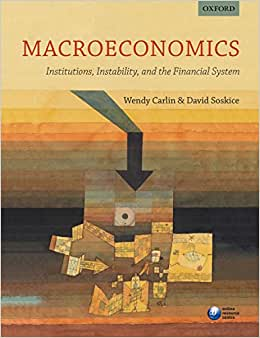
\includegraphics[width=0.25\textwidth]{./figures/carlin}} \qquad
        \subfloat[Challe (2019)\label{fig1b}]{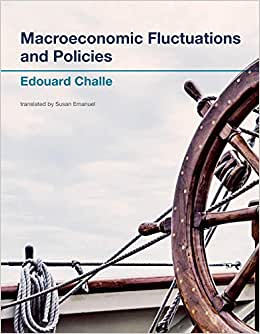
\includegraphics[width=0.25\textwidth]{./figures/challe}} \qquad
        \subfloat[Blanchard (2017)\label{fig1c}]{
\includegraphics[width=0.25\textwidth]{./figures/blanchard}}
        \caption{Bibliografia do curso}
        \label{fig1}
    \end{figure}
\end{frame}

\begin{frame}{Bibliografia}
    \begin{figure}        
        \centering
        \subfloat[Froyen (2013)\label{fig2a}]{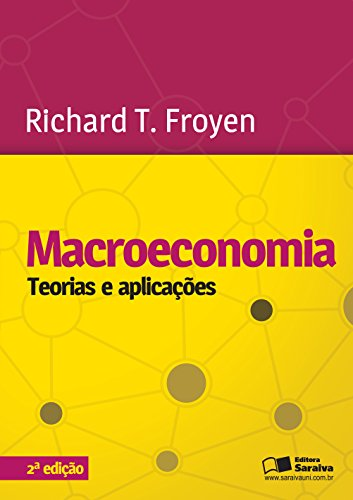
\includegraphics[width=0.25\textwidth]{./figures/froyen}} \qquad
        \subfloat[Dornbusch et al. (2013)\label{fig2b}]{
\includegraphics[width=0.25\textwidth]{./figures/dornbusch}} \qquad
        \subfloat[Abel et al. (2008)\label{fig2c}]{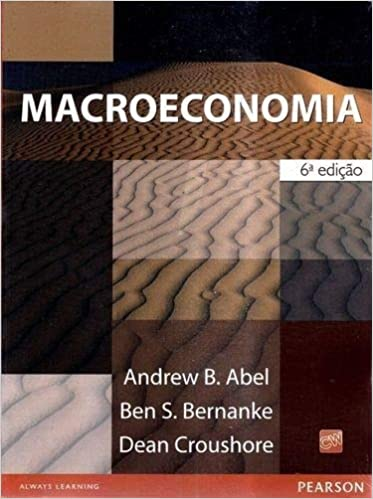
\includegraphics[width=0.25\textwidth]{./figures/bernanke}}
        \caption{Bibliografia do curso}
        \label{fig2}
    \end{figure}
\end{frame}

\begin{frame}{Bibliografia}
    \begin{figure}
        \centering
        \subfloat[Snowdon e Vane (2005)\label{fig3a}]{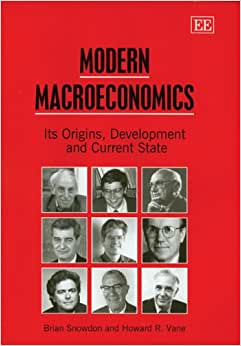
\includegraphics[width=0.25\textwidth]{./figures/snowdon}} \qquad
        \subfloat[Mankiw (2021)\label{fig3b}]{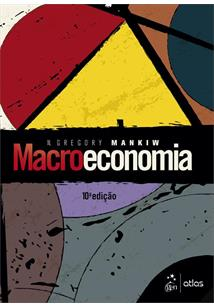
\includegraphics[width=0.25\textwidth]{./figures/mankiw}} \qquad
        \subfloat[Alem (2018)\label{fig3c}]{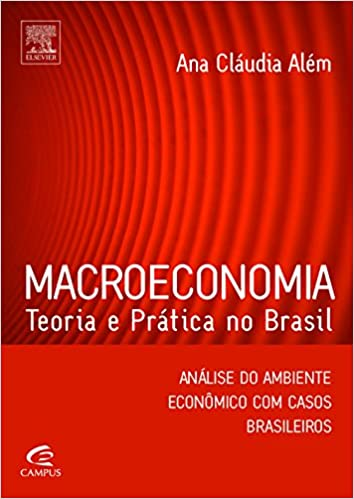
\includegraphics[width=0.25\textwidth]{./figures/alem}}
        \caption{Bibliografia do curso}
        \label{fig3}
    \end{figure}
\end{frame}

\begin{frame}{Bibliografia}
    \begin{figure}
        \centering
        \subfloat[Lopes e Vasconcellos (2008)\label{fig4a}]{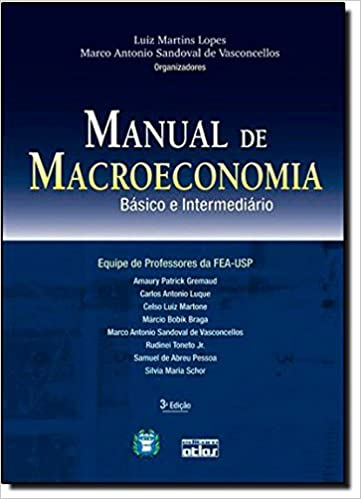
\includegraphics[width=0.25\textwidth]{./figures/lopes}} \qquad
        \subfloat[Simonsen e Cysne (2009)\label{fig4b}]{
\includegraphics[width=0.25\textwidth]{./figures/simonsen}} \qquad
        \subfloat[Scarth (1988)\label{fig4c}]{
\includegraphics[width=0.25\textwidth]{./figures/scarth}}
        \caption{Bibliografia do curso}
        \label{fig4}
    \end{figure}
\end{frame}

\begin{frame}{Bibliografia}
    \begin{itemize}
        \footnotesize
        \item ABEL, A.; BERNANKE, B.; CROUSHORE, D. \emph{Macroeconomia}. 6.ed. Pearson Prentice Hall, 2008.
        \item ALEM, A. \emph{Macroeconomia: teoria e prática no Brasil}. 2.ed. Rio de Janeiro: Elsevier, 2018. Disponível em: \href{https://app.minhabiblioteca.com.br/books/9788595152083}{app.minhabiblioteca.com.br/books/9788595152083}
        \item BLANCHARD, O. \emph{Macroeconomia}. 7.ed. São Paulo: Pearson Education do Brasil, 2017.
        \item CARLIN, W.; SOSKICE, D. \emph{Macroeconomics: Institutions, instability, and the financial system}. Oxford, UK: Oxford University Press, 2015.
        \item CHALLE, E. \emph{Macroeconomic fluctuations and policies}. Cambridge, MA: The MIT Press, 2019.
        \item DORNBUSCH, R.; FISCHER, S.; STARTZ, R. \emph{Macroeconomia}. 11.ed. Porto Alegre: AMGH, 2013. Disponível em: \href{https://app.minhabiblioteca.com.br/books/9788580551853}{app.minhabiblioteca.com.br/books/9788580551853}
        \item FROYEN, R. \emph{Macroeconomia: teorias e aplicações}. 2.ed. São Paulo: Saraiva, 2013. Disponível em: \href{https://app.minhabiblioteca.com.br/books/9788502175235}{app.minhabiblioteca.com.br/books/9788502175235}
        \item LOPES, L.M.; VASCONCELLOS, M.A.S. \emph{Manual de Macroeconomia: Nível básico e nível intermediário}. 3.ed. São Paulo: Atlas, 2008.
        \item MANKIW, G. \emph{Macroeconomia}. 10.ed. Rio de Janeiro: Atlas, 2021. Disponível em: \href{https://app.minhabiblioteca.com.br/reader/books/978-85-216-2749-4/}{app.minhabiblioteca.com.br/reader/books/978-85-216-2749-4}
        \item SCARTH, W.M. \emph{Macroeconomics: An introduction to advanced methods}. Toronto: Harcourt Brace Jovanovich Canada Inc., 1988. (Tradução: Sergio da Silva).
        \item SIMONSEN, M.H.; CYSNE, R.B. \emph{Macroeconomia}. 4.ed. São Paulo: Atlas, 2009. Disponível em: \href{https://app.minhabiblioteca.com.br/reader/books/9788522465330}{app.minhabiblioteca.com.br/reader/books/9788522465330}
        \item SNOWDON, B.; VANE, H.R. \emph{Modern Macroeconomics: its Origins, Development and Current State}. Northampton, MA: Edward Elgar, 2005.
    \end{itemize}
\end{frame}
\end{document}